% Chapter 4

\chapter{Architecture} % Main chapter title

\label{chap:Chapter4} % For referencing the chapter elsewhere, use \ref{chap:Chapter4} 

%----------------------------------------------------------------------------------------

This chapter details on the practical implementation of the proposed algorithm. It begins with an overview in Section 4.1, which outlines the key methods and tools used throughout the development process. Section 4.2 dives into the detailed steps taken to develop the algorithm, including both hardware and software components, as well as the various tools and libraries (crates) employed. Section 4.3 then describes the algorithm designed to select the best SVs and presents the results of this selection process. This chapter provides a comprehensive view of how the theoretical concepts were translated into a working solution.

\section{Overview}

The demand for an algorithm that selects the optimal analog signal has grown alongside the increasing adoption of merging units in substations. As substations transition to digitalization, merging units become indispensable for ensuring efficient performance. These units play a critical role by making various other substation components dependent on their technology. Previously, the only critical protocol was GOOSE, used for transmitting trip signals and equipment interlocks. Now, with the adoption of merging units, the communication network itself becomes critical. It ensures the accurate reception of analog signals from CTs and VTs, allowing protection algorithms to promptly identify network faults.

Consequently, formerly non-critical equipment like switches must now meet stringent performance criteria to prevent delays. This necessitates the implementation of PTP across all critical network devices, establishing PTP as the master clock for the entire substation network.

Merging units are ushering substations into the digital age, yet they also introduce new challenges. In older substations, concerns about analog signals were limited to issues like broken wires and induction. Today, with numerous interconnected devices requiring precise timing and high performance, ensuring proper system operation becomes crucial.

\section{Hardware Setup}

For the development and execution of this project, a Dell Inspiron personal computer has been utilized. This machine is equipped with robust specifications to support the complex computational and networking requirements of the research. The key features of this computer are as follows:

\begin{itemize}
	\item Processor: Intel Core i5 10th Generation, offering a balanced blend of performance and efficiency for handling various computational tasks required during the development and testing phases.
	\item Memory: 8 GB of RAM, providing sufficient memory capacity to run multiple applications and perform intensive data processing operations seamlessly.
	\item Networking: The system includes two Ethernet cards to facilitate network connectivity:
	Integrated Ethernet Card: The built-in Ethernet card that comes with the computer.
	Gigabit USB to Ethernet Adapter: An additional gigabit Ethernet adapter connected via USB, enhancing the computer’s networking capabilities.
	Network Speed Limitation: Despite the presence of a gigabit Ethernet adapter, the overall system network speed is limited to 100 Mbits/s. This is due to the maximum speed supported by the jetson nano, which is being used in conjunction with the Dell Inspiron for this project.
\end{itemize} 

The Jetson Nano stands out for its versatility and compact design, making it an ideal choice for deploying sophisticated algorithms in research projects. Key features include:

\begin{itemize}
	\item Processing Power: Equipped with a 1.43 GHz quad-core ARM Cortex-A57 processor and a 128-core NVIDIA Maxwell GPU, offering robust computational capabilities necessary for real-time data processing and algorithm execution.
	\item Memory: Includes 4 GB of LPDDR4 RAM, ensuring efficient storage and retrieval of data crucial for running complex algorithms and maintaining system responsiveness.
	\item Connectivity: Integrated with Gigabit Ethernet, enabling high-speed wired communication essential for modern substation automation applications, and also an ethernet adapter using USB3.0 with gigabit connection.
	\item GPIO Pins: Equipped with a 40-pin GPIO header, allowing direct interfacing with external sensors, actuators, and other peripherals, which is indispensable for hardware integration in substation environments.
\end{itemize}

The specifications of the Dell Inspiron ensure it can manage the comprehensive demands of the research, ranging from the development and testing of algorithms to interfacing with the Jetson Nano for real-time data processing and network simulations. Equipped with an Intel Core i5 10th Generation processor and 8 GB of RAM, this personal computer provides the necessary performance and memory capacity for running complex applications and intensive data operations. The inclusion of dual Ethernet cards—one integrated and one gigabit USB to Ethernet adapter—enables flexible and reliable network configurations, essential for accurately emulating substation environments and conducting thorough testing.

The Jetson Nano is equally well-suited for executing the algorithm designed to optimize SV selection in substation automation systems. Its powerful ARM processor and NVIDIA GPU offer robust computational capabilities and efficient data handling. The integrated Gigabit Ethernet facilitates high-speed wired communication, while the 40-pin GPIO header allows for direct interfacing with external sensors and actuators. Despite the network speed being limited to 100 Mbits/s due to the maximum capacity of certain interfaces, these features collectively ensure reliable performance and effective integration into research and development efforts.

By harnessing the strengths of both the Dell Inspiron and the Jetson Nano, this research project benefits from a synergistic blend of hardware capabilities. The Dell Inspiron serves as a robust foundation for development, testing, and executing the algorithm, leveraging its computational power and memory capacity. Meanwhile, the Jetson Nano operates as both a merging unit and a protection relay, demonstrating its adaptability and connectivity. This dual functionality makes the Jetson Nano an optimal platform for handling real-time data processing and network simulations. Together, these platforms play a pivotal role in advancing substation automation, improving operational efficiency, and bolstering the reliability of substation systems.

\section{Software Technologies}

The software development process began with selecting the programming language for developing the algorithm. Today, we have many languages that meet performance needs and are widely used in the market, such as C and C++. These languages prioritize performance, which is why they are predominantly used in embedded systems. However, we also have languages that are easier to develop and write, although not as performant, such as Python/MicroPython.

After thoroughly analyzing the scenario in which my development needed to be inserted, I came across the Rust language. Rust offers performance comparable to C and C++ but without the memory management issues inherent to these languages. Given that this development is related to critical systems, I opted to use a safer language. Thus, the development was carried out in Rust.

The decision to use Rust was also influenced by its modern design principles and strong community support. Rust’s ownership model ensures memory safety and eliminates common bugs such as null pointer dereferencing and buffer overflows. This is particularly important in critical systems where reliability and safety are essential.

Furthermore, Rust's rich type system and pattern matching capabilities facilitate the development of robust and maintainable code. The language's concurrency model is designed to prevent data races, making it a suitable choice for applications requiring high performance and safety.

By choosing Rust, the development process benefits from both high efficiency and enhanced safety, ensuring that the algorithm operates reliably within the substation automation system. This strategic choice underscores the commitment to using cutting-edge technologies to achieve optimal performance and reliability in critical system applications.

\subsection{Cargo}

Cargo is Rust's official package manager and build system, integral to managing Rust projects. It simplifies the process of managing dependencies, compiling code, running tests, and creating documentation. Here's an overview of Cargo's key features:

\begin{itemize}

	\item Dependency Management
	\begin{itemize}
		\item Crates: Cargo allows developers to easily include third-party libraries (known as crates) into their projects. These crates are listed in a Cargo.toml file, where you can specify the version of each dependency.
		\item Automatic Resolution: Cargo automatically fetches and compiles these dependencies, ensuring that the correct versions are used, and resolving any conflicts between different versions of the same crate.
	\end{itemize}

	\item Build and Compilation
	\begin{itemize}
		\item Automatic Resolution: Cargo automatically fetches and compiles these dependencies, ensuring that the correct versions are used, and resolving any conflicts between different versions of the same crate.
		\item Cross-Compilation: Cargo supports cross-compilation, allowing developers to build their Rust projects for different target platforms, which is particularly useful for embedded systems.
	\end{itemize}

	\item Project Management
	\begin{itemize}
		\item Project Initialization: Starting a new Rust project is simple with Cargo. By running cargo new 'project name', Cargo automatically creates a new directory with a basic Rust project structure, including the necessary Cargo.toml file and a default source directory.
		\item Workspaces: Cargo supports workspaces, enabling the management of multiple related packages within a single repository. This is particularly useful for large projects with multiple components that need to be developed and managed together.
	\end{itemize}

	\item Community and Ecosystem
	\begin{itemize}
		\item Crates.io: Cargo is tightly integrated with Crates.io, the Rust community's official crate registry. This allows developers to publish their libraries and applications, making them available to others in the community.
		\item Cargo.lock: Cargo manages a Cargo.lock file that records the exact versions of all dependencies used in a project, ensuring consistency across different builds and environments.
	\end{itemize}
\end{itemize}

Cargo's function in the Rust ecosystem is fundamental, as it provides a unified way to manage the entire lifecycle of a Rust project—from development and dependency management to testing, documentation, and deployment. Its user-friendly interface and powerful features make it an essential tool for Rust developers, facilitating a smooth and efficient development process.

\subsection{Crates}
Crates in Rust are the building blocks of Rust projects and packages. A "crate" refers to a compilation unit in Rust and can be a library or a binary.

\begin{itemize}
	
	\item Types of Crates
	\begin{itemize}
		\item Binary Crates: These are executable applications. When you create a binary crate, it generates a single executable file.
		\item Example: If you write a Rust program with a main.rs file, it’s a binary crate because it compiles to an executable.
		\item Library Crates: These contain reusable code that other projects can depend on. Instead of producing an executable, a library crate compiles to a .rlib file that other projects can link against.
		\item Example: A collection of utility functions or algorithms that you can share across multiple projects.
	\end{itemize}
	
	\item Crates.io
	\begin{itemize}
		\item Crates.io is the official Rust package registry where developers can publish and share their library crates. It's similar to npm for Node.js or PyPI for Python.
		\item Developers can search for and download crates published by others, integrating them into their projects with ease.
	\end{itemize}
	
	\item Dependency Management with Crates
	\begin{itemize}
		\item In Rust, projects can depend on other crates. You specify these dependencies in the Cargo.toml file, which lists all the crates your project needs, along with their versions.
		\item Cargo, Rust’s package manager, handles fetching these dependencies from Crates.io, ensuring compatibility and managing versions.
	\end{itemize}
	
	\item Benefits of using Crates
	\begin{itemize}
		\item Modularity: Crates encourage modular design, making it easy to split a project into smaller, reusable components. Each crate can be developed, tested, and compiled independently. needs, along with their versions.
		\item Reusability: By using crates, you can leverage existing solutions for common problems. Whether it's handling dates, parsing JSON, or working with databases, there’s likely a crate for it.
		\item Dependency Management: Cargo automatically manages dependencies, ensuring that you’re using the correct versions of the crates your project depends on, thus avoiding compatibility issues.
	\end{itemize}
	
	\item Community and Ecosystem
	\begin{itemize}
		\item The Rust community actively contributes to the ecosystem by publishing high-quality crates on Crates.io. This makes it easier for developers to find reliable, well-maintained packages for their projects.
	\end{itemize}
\end{itemize}

In this project, I am exclusively using library crates, which are essential to the development process. These libraries significantly streamline the development work and provide crucial functionality. Additionally, by managing these libraries with Cargo, I can easily track and control the versions I’m using, ensuring consistency throughout the project.

Crates are central to the Rust ecosystem, promoting code reuse, modularity, and collaboration. Whether you’re building a small utility or a large-scale application, crates help structure your project and tap into the wealth of libraries and tools available in the Rust community. Below, I’ll describe the most important libraries that have been integral to this development.

\subsection{Tokio Crate}

Tokio\footnote{\url{https://crates.io/crates/tokio}} is one of the most popular and robust asynchronous runtimes in the Rust ecosystem, offering essential components for building high-performance, reliable, and scalable network applications. Leveraging Rust’s concurrency model, Tokio provides an event-driven, non-blocking I/O system that allows developers to handle thousands of concurrent connections with minimal overhead. This is particularly beneficial for applications that perform extensive I/O operations, such as reading from or writing to sockets, without needing to wait for these operations to complete before continuing with other tasks.

In addition to its asynchronous runtime, Tokio includes a comprehensive set of utilities such as timers, channels, and synchronization primitives, which are invaluable in managing complex concurrent systems. Its seamless integration with Rust's async/await syntax significantly simplifies the development of asynchronous code, making it more readable and maintainable.

A key feature of Tokio is its advanced multithreaded, work-stealing task scheduler, which is critical for optimizing the performance of asynchronous applications in Rust. This scheduler distributes tasks efficiently across multiple threads, ensuring full utilization of available CPU cores. By using a work-stealing approach, Tokio ensures that no single thread becomes a performance bottleneck. If one thread finishes its tasks while others are still occupied, it can "steal" tasks from the busy threads, leading to a more balanced and efficient distribution of workload.

This design is particularly beneficial in scenarios where an application must manage a large number of concurrent operations, such as handling network connections or processing real-time data streams. The scheduler minimizes idle time and maximizes throughput, which is essential for maintaining high-performance levels in demanding applications. Additionally, by automatically balancing the load, the scheduler reduces the need for manual optimization, allowing developers to concentrate on the core logic of their applications rather than focusing on performance tuning across threads. This makes Tokio an ideal choice for building scalable and responsive systems in Rust.

Tokio has to offer essential tools for managing concurrency and parallelism efficiently like:

\begin{itemize} 
	\item Concurrency and Parallelism: Tokio enables the handling of numerous tasks concurrently, facilitating the development of highly efficient and responsive applications. By utilizing asynchronous programming, Tokio helps manage multiple operations simultaneously without blocking the execution of other tasks. 
	\item Asynchronous I/O: Tokio excels in non-blocking I/O operations, making it ideal for applications that need to handle multiple network connections concurrently. This is particularly relevant for the merging unit and protection relay functions in this project. 
	\item Scalability: With Tokio, systems can scale efficiently, handling increased loads without a significant decline in performance. This is especially important for real-time data processing and network simulations required in substation automation systems.
\end{itemize}

By incorporating Rust and leveraging the Tokio crate, the development process benefits from high efficiency and enhanced safety, ensuring that the algorithm functions reliably within the substation automation system. This strategic choice highlights the commitment to using cutting-edge technologies to deliver optimal performance and reliability in critical system applications.

\subsection{Serde Crate}

Serde\footnote{\url{https://crates.io/crates/serde}} is the standard crate for serialization and deserialization in Rust, offering a flexible and highly efficient framework for converting complex data structures to and from various formats, such as JSON, TOML, YAML, and more. Serialization is the process of converting a data structure into a format that can be stored or transmitted, while deserialization is the reverse operation. Serde's performance is one of its standout features; it’s designed to minimize overhead and maximize speed, making it suitable for high-performance applications where data exchange is frequent and data structures are large or complex.

Serde ecosystem is extensive, with support for a wide range of data formats and seamless integration with other Rust crates. The framework is highly extensible, allowing developers to define custom serialization and deserialization logic for their data types. This flexibility ensures that Serde can handle nearly any data representation need, whether it's a simple JSON API or a complex, nested configuration file. Furthermore, Serde derive macros (\texttt{\#\textbackslash{}derive(Serialize, Deserialize)}) make it incredibly easy to implement serialization and deserialization for Rust structs and enums, saving developers from writing boilerplate code.

\subsection{Crc32Fast Crate}

Crc32Fast\footnote{\url{https://crates.io/crates/crc32fast}} is a high-performance crate designed to compute CRC-32 checksums efficiently. CRC-32 (Cyclic Redundancy Check) is a widely used algorithm for detecting errors in data transmission or storage. It’s a lightweight but powerful tool that can quickly determine if data has been corrupted, making it indispensable in contexts like file integrity checks, network communications, and data archival. The crc32fast crate is optimized for speed, using techniques like loop unrolling and SIMD (Single Instruction, Multiple Data) instructions to process data in parallel, significantly speeding up checksum computations.

This crate is particularly useful in applications where performance is critical, such as systems that handle large volumes of data or require real-time error detection. For example, in networking, CRC-32 checksums are often used to ensure that packets are received without errors. By integrating crc32fast into such a system, developers can maintain high throughput while ensuring data integrity. Additionally, its simplicity and efficiency make it a go-to choice for Rust developers needing a reliable method for error-checking large datasets or streams.

\subsection{Pnet Crate}

Pnet\footnote{\url{https://crates.io/crates/pnet}} (Packet Network) is a low-level networking crate in Rust that provides extensive capabilities for crafting, sending, and receiving raw network packets. It offers granular control over network communications, making it an essential tool for developers working on networking protocols, network security applications, or custom network infrastructure. Pnet allows you to build and dissect packets for various network layers (Ethernet, IP, TCP/UDP, etc.), giving you the ability to create highly customized network interactions that go beyond what standard networking libraries offer.

One of Pnet's key strengths is its flexibility. It supports a wide range of protocols and can be used for tasks like network monitoring, building packet sniffers, creating custom firewall rules, or even developing your own network protocol. Additionally, Pnet is well-integrated with Rust’s safety guarantees, meaning you can perform low-level network programming with fewer risks of common bugs, such as buffer overflows or memory leaks. This makes Pnet an excellent choice for developers who need both the power of low-level networking and the safety of Rust.

\subsection{Log Crate}

Log\footnote{\url{https://crates.io/crates/log}} is a logging facade for Rust that provides a simple and flexible way to capture log messages in your applications. It’s designed to be lightweight and minimal, focusing on defining a standard logging API that libraries and applications can use without committing to a specific logging implementation. This approach allows you to write code that logs messages at various levels (error, warn, info, debug, trace) and later decide how those logs are handled, whether they're printed to the console, written to a file, or sent to a logging service.

The log crate’s primary advantage is its decoupling of log producers from log consumers. You can use the log macros (log!, info!, error!, etc.) throughout your codebase, and then choose or implement a logging backend (like env\_logger or slog) that suits your application's needs. This flexibility makes log an ideal choice for libraries, as it allows the library to emit logs without enforcing a specific logging behavior on the end user. As a result, the log crate has become a standard in the Rust ecosystem, used by many libraries and applications to ensure consistent and configurable logging.

\subsection{Env\_Logger Crate}

Env Logger\footnote{\url{https://crates.io/crates/env_logger}} is a simple but powerful logging backend for the log crate, designed to configure logging via environment variables. This crate is particularly useful in situations where you need to adjust the verbosity of logging without modifying the code itself, such as in different deployment environments (development, testing, production). By setting environment variables, you can control which log levels are enabled and where the log output is directed, making env\_logger extremely flexible and easy to use.

For example, in a production environment, you might want to only log warnings and errors, while in a development environment, you might enable debug and trace logs to troubleshoot issues. Env\_logger supports these scenarios by allowing you to configure log levels on a per-module basis, providing granular control over the logging output. This makes it an invaluable tool for developers who need to maintain visibility into their applications’ behavior across different environments without cluttering the codebase with log configuration details.

\subsection{Chrono}

Chrono\footnote{\url{https://crates.io/crates/chrono}} is a comprehensive and robust date and time library for Rust, offering a rich set of features for working with dates, times, and time zones. It’s designed to be easy to use yet powerful enough to handle complex date and time manipulations. Chrono allows you to parse and format date/time strings, perform arithmetic operations on dates and times (e.g., adding or subtracting time durations), and work with time zones, including conversions between UTC and local times.

One of Chrono's most significant advantages is its flexibility and precision, making it suitable for a wide range of applications. Whether you need to manage timestamps in a database, schedule tasks, log events, or handle time-sensitive operations in a global application, Chrono provides the tools you need. It also supports custom date and time formats, allowing you to work with both standard and non-standard representations of time. Chrono is widely adopted in the Rust ecosystem for any application that requires accurate and reliable date/time handling.

\section{Solution Design}

This thesis proposes a method for selecting the best analog/digital signal sent by multiple Merging Units. The signal is initially analog because it is acquired in that form from VT and CT, but the Merging Unit converts it into a digital signal following the IEC-61850-9-2 protocol. The device proposed in this work receives the digital signal, compares it with another one that's come from another Merging Unit. After this comparison, an algorithm implemented using a state machine selects which signal will be forwarded to the protection systems subscribing to these SV.

To achieve this, it was necessary to develop and implement the IEC~61850-9-2 protocol from the ground up. Since there is no available library for the RUST programming language, one had to be created. As a result, a publisher, a subscriber, and the core algorithm which is the main focus of this thesis were developed. This algorithm must receive information from two Merging Units and, after processing it, send the selected data to the protection system.

Figure~\ref{fig:overview_of_implementation} The components of the thesis are interconnected as follows: Two MUs send data to the algorithm. The algorithm then evaluates the information from both MUs, selects the most optimal data, and transmits it to the Protection Relay. This selection process ensures that the Protection Relay receives the best possible data based on the criteria defined by the algorithm.

\begin{figure}[tbh]
	\centering
	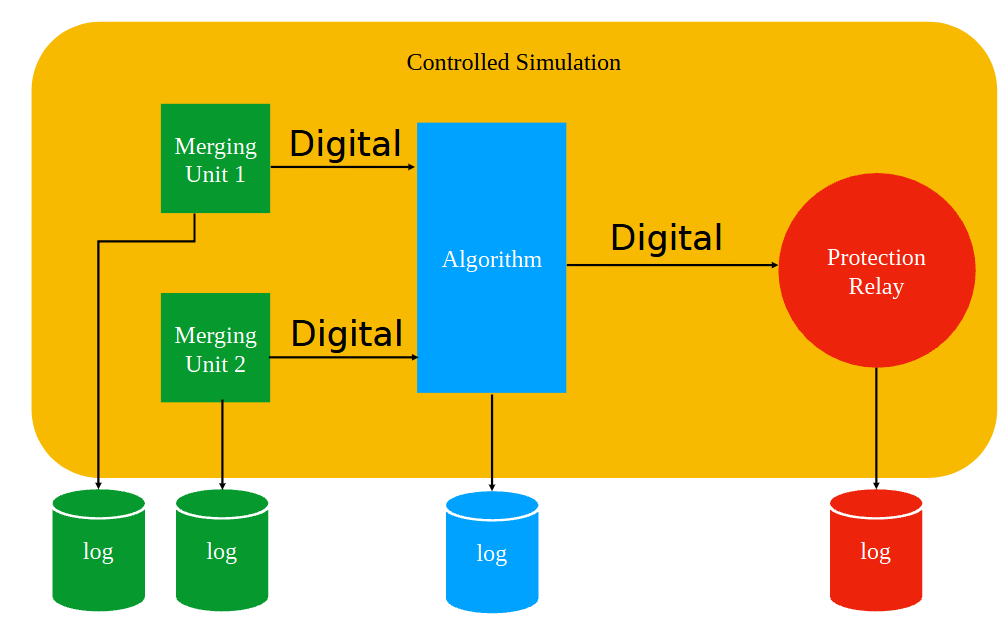
\includegraphics[width=0.80\textwidth, keepaspectratio]{ch4/assets/Implementation.png} % Reduce to 90% of the text width
	\caption{How the implementation was designed to work.}
	\label{fig:overview_of_implementation}
\end{figure}
\FloatBarrier

%\raggedright
The development process began with the creation of the publisher, a software that emulates the operation of a Merging Unit. This software was built in accordance with the standard IEC~61850-9-2 for SV packets.

Figure~\ref{fig:sv_packet} shows the frame structure of a Sampled Value (SV) Packet~\footnote{\url{https://www.typhoon-hil.com/documentation/typhoon-hil-software-manual/References/iec_61850_sampled_values_protocol.html}}.

\begin{figure}[tbh]
	\centering
	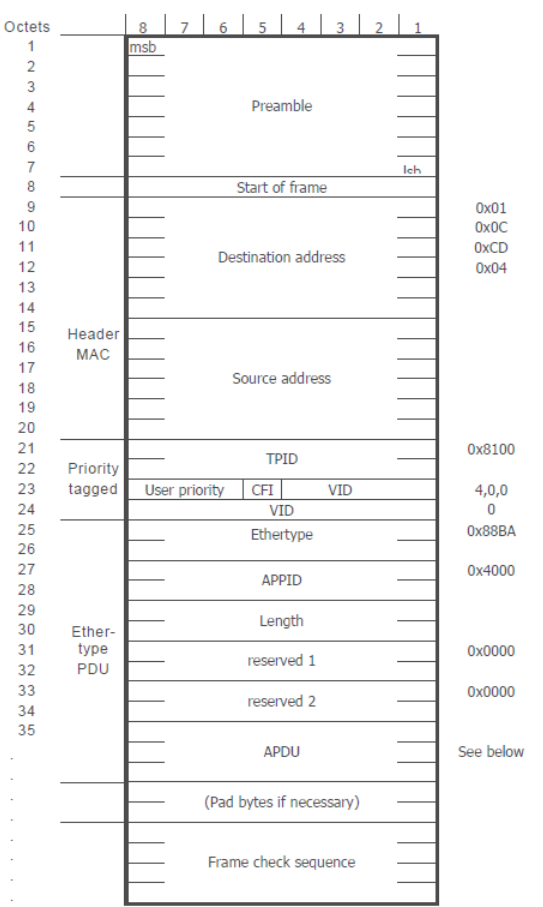
\includegraphics[width=0.75\textwidth, keepaspectratio]{ch4/assets/SV_Packtes.png} % Reduce to 90% of the text width
	\caption{How is constructed a Sampled Values Packet following the standard IEC~61850-9-2 (Image credits: Typhoon HIL)}
	\label{fig:sv_packet}
\end{figure}
\FloatBarrier


Once the packet structure was defined, a function was created to calculate the values to be sent along with the SVs. This function uses the current execution time to generate similar values between the two Merging Units.

We also implemented verification and validation of the packets using Cyclic Redundancy Check (CRC). The CRC is added to the SV packet during its creation, and on the subscriber side, it is verified to ensure the packet's validity.

The second phase of development focused on the subscriber. Upon receiving the packet over the Ethernet network, and in compliance with the IEC~61850-9-2 protocol standards, the packet is reconstructed, its integrity validated using CRC, and the relevant information extracted and logged. The subscriber device we developed acts as a protection relay, where the received information is converted back to an analog signal and applied to the relay’s protection algorithms.

The third phase centered on developing the algorithm for selecting the best SV. This selection process involves analyzing the values received in the SV packets. To achieve this, we implemented an SV subscriber capable of retrieving data transmitted via this protocol, utilizing components from the earlier development stages. After receiving the data via Ethernet, the information is extracted, evaluated, and the best signal is chosen between the packets sent by Merging Unit 1 and Merging Unit 2. Once the best signal is identified, it is sent using the SV publisher, thus completing the development process aligned with the thesis's objectives.

The algorithm utilizes the Tokio crate, which provides a work-stealing task scheduler, allowing for concurrent and parallel processing. This enables the immediate retransmission of packets from the Merging Unit with the better signal, with the algorithm switching only when another Merging Unit provides a superior analog signal. This approach ensures real-time performance, essential for the required application.

This thesis specifically addresses scenarios involving two Merging Units. Although the case of more than two Merging Units was not considered, the algorithm can be adapted to handle such situations.
	
\section{Algorithm Description}

The description of the algorithm hinges on a deep understanding of both the publisher and subscriber functions. The aim is to create an algorithm capable of selecting the optimal samples from two independent devices that measure the same electrical quantity. This involves transmitting these measurements via a protocol, decompressing the data, extracting the necessary values, evaluating them, and ultimately selecting the best sample. All of this must be accomplished within a timeframe that ensures the SVs reach the protection devices without delay each SV being transmitted every 250 microseconds.

The algorithm is triggered upon the reception of an SV from one of the merging units. Once received, the SV is processed and evaluated to determine whether it is valid, invalid, or questionable. If the sample is valid, its values are extracted for comparison with those from the other merging unit. In the case of an invalid or questionable sample, it is excluded from the value acquisition process. However, the algorithm keeps track of the number of invalid samples, which is one of the criteria used to decide whether to switch the SVs being sent to the protection relays.

For valid samples, a comparison is made on a sample-by-sample basis to ensure the best result. If the error does not exceed 25\%, the current SV is maintained; however, if the error surpasses 25\%, the SV being sent to the protection relays is switched. A state machine was implemented to make the decision on which SV to send to the protection devices. Although the system receives values from two merging units, only one of the two received SVs is transmitted.

The state machine processes all incoming SV frames according to the logic outlined below.

Figure~\ref{fig:state_machine} Here has a representation of the state machines it was implemented to make a decision which SV's is going to send. 

\begin{figure}[tbh]
	\centering
	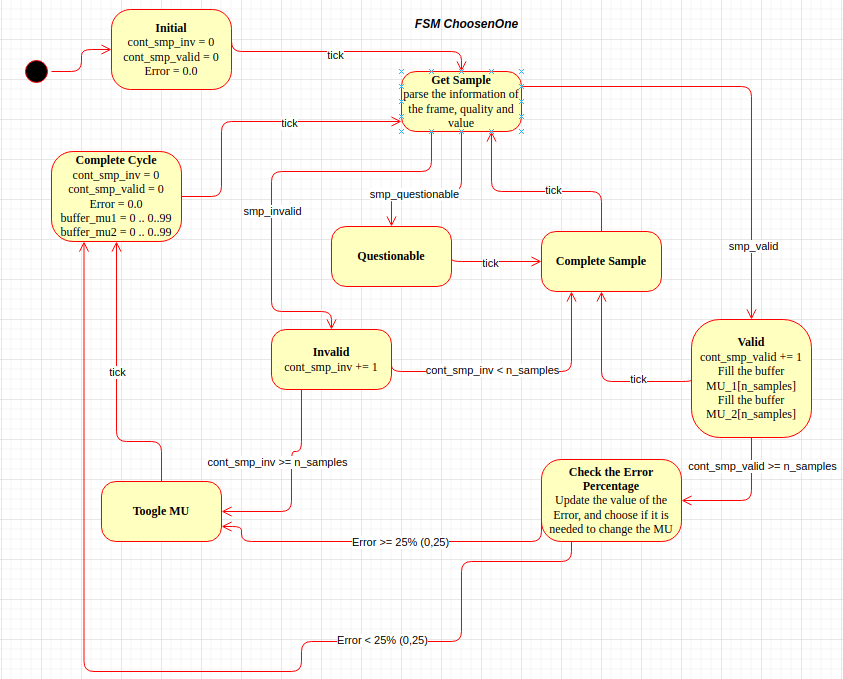
\includegraphics[width=0.95\textwidth, keepaspectratio]{ch4/assets/state_machine.png} % Reduce to 90% of the text width
	\caption{State Machine of Decision Make.}
	\label{fig:state_machine}
\end{figure}
\FloatBarrier

The state machine is implemented in Rust and operates using two mechanisms for state transitions: events and ticks. Events are specific actions that trigger progress within the state machine, while ticks represent units of time. When a specified time elapses and the state requires only a tick to proceed, the machine advances, similar to how it transitions in response to events.
\begin{itemize}
	\item Initial State: This state runs only once when the algorithm is first executed. After this, the state can only be re-entered by a reset. After a tick, the state machine transitions to the 'Get Sample' state.
	\item Get Sample: In this state, the sample data is received, and information about the packet is processed. Based on the packet’s validity, the state machine decides to transition to one of three states: Valid, Invalid, or Questionable. The packet's status (valid, questionable, or invalid) determines the next state.
	\item Questionable: In the 'Questionable' state, no further action is taken other than validating the received packet. After a tick, the machine moves to the 'Complete Sample' state.
	\item Invalid: In the 'Invalid' state, the machine checks whether the number of valid packets received is below a defined threshold (n\_samples). If so, it advances to the 'Complete Sample' state; otherwise, it transitions to the 'Toggle MU' state.
	\item Valid: In the 'Valid' state, the system checks if the number of valid packets is below the threshold (n\_samples). If so, it transitions to the 'Complete Sample' state; otherwise, it moves to 'Check Error Percentage'. Additionally, the sample is placed in the appropriate index of the buffer, corresponding to the three-phase and neutral current and voltage measurements (Phase A to N) for the two MUs (Merging Units).
	\item Complete Sample: This state is essentially a waiting period, where the machine waits for a tick before transitioning back to the 'Get Sample' state.
	\item Toggle MU: In the 'Toggle MU' state, the Merging Unit is toggled, and the machine waits for a tick before transitioning to the 'Complete Cycle' state.
	\item Check Error Percentage: In this state, the entire buffer is evaluated to calculate the error percentage. If the error is below 25\%, the machine remains in the same MU and moves to the 'Complete Cycle' state. If the error exceeds 25\%, it transitions to the 'Toggle MU' state.
	\item Complete Cycle: In the 'Complete Cycle' state, all variables are reset to begin a new cycle of the algorithm. After resetting, the machine waits for a tick to return to the 'Get Sample' state.
\end{itemize}

This state machine ensures efficient processing and evaluation of sampled values from the Merging Units, adapting dynamically based on packet validity and system performance thresholds.

\begin{lstlisting}[caption={State Machine struct.}]
// Define the state machine
struct FrameProcessor {
	state: State,
	cont_smp_inv: u32,
	cont_smp_valid_sv_id_1: u32,
	cont_smp_valid_sv_id_2: u32,
	error_percentage: f32,
	buffer_mu1: [[i32; N_SAMPLES as usize]; 8], // buffer MU 1 current A,B,C and N - voltage A,B,C and N
	buffer_mu2: [[i32; N_SAMPLES as usize]; 8], // buffer MU 2 current A,B,C and N - voltage A,B,C and N
	toggle_mu: bool,
}
impl FrameProcessor {
	fn new() -> Self {
		Self {
			state: State::Initial,
			cont_smp_inv: 0, // Initialize cont_invalid
			cont_smp_valid_sv_id_1: 0,
			cont_smp_valid_sv_id_2: 0,
			error_percentage: 0.0,
			buffer_mu1: [[0 ; N_SAMPLES as usize]; 8],
			buffer_mu2: [[0 ; N_SAMPLES as usize]; 8],
			toggle_mu: false,
			
		}
	}
\end{lstlisting}

The diagram in Figure~\ref{fig:test_setup} illustrates the deployment of the software components on the hardware platforms.
The Merging Units and Protection Relay are simulated on the Jetson Nano node, while the Algorithm runs on the PC.
An Ethernet link connects the Merging Units to the Algorithm, and another Ethernet link connects the Algorithm to the Protection Relay.

The workflow is as follows:
\begin{enumerate}
	\item The MUs send sampled values (SV) to the Algorithm.
	\item The Algorithm analyses the received data and adaptively selects the best source.
	\item The Algorithm forwards the SV to the Protection Relay.
\end{enumerate}


\begin{figure}[tbh]
	\centering
	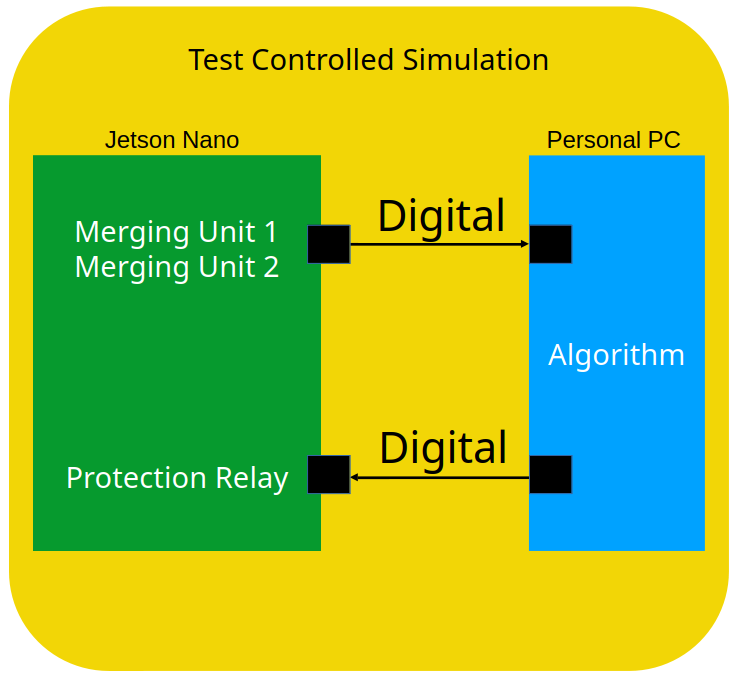
\includegraphics[width=0.95\textwidth, keepaspectratio]{ch4/assets/test_setup.png}
	\caption{How is connected the two simulators of SV's to exchange the information.}
	\label{fig:test_setup}
\end{figure}
\FloatBarrier

All information regarding the development is available on GitHub, along with additional resources in the following location:

\hspace{1cm} \url{https://github.com/everton-oriente/IEC61850_9_2_SV}

% COMENTADO POR AMB
%These platforms collectively provide comprehensive access to the project's documentation, source code, and related materials.


\begin{comment}


\subsection{Results}

Leading the development and implementation of a communication protocol like IEC~61850-9-2 presented a completely different challenge. It required me to ensure that any other equipment connected to the network could understand exactly what was being sent. This involved understanding how operating systems handle network packets, the various headers that are added to ensure the information is properly routed and delivered to the correct destination, and how to assemble SV packets. The packets had to be sent in a way that the receiving application could correctly reassemble and interpret the data after it had been converted into bytes. This process required not only receiving and converting the bytes back into usable information within the IEC~61850-9-2 protocol but also ensuring that the destination equipment could understand the payload. Furthermore, it was critical to verify that the packet was intact and suitable for content analysis, while also maintaining synchronization between the two applications. This was particularly important given that the information needs to be transmitted every 250 microseconds, making network latency a critical factor.

The results obtained after all phases of development were satisfactory, considering the existing conditions. We used the Network Time Protocol (NTP) as the master clock, which provides a precision of 1 millisecond. However, achieving 100\% accuracy in timing was challenging because the protocol itself has a precision that exceeds the 250-microsecond interval at which we were transmitting the SV packets. Despite this limitation, the tests yielded values that were close to what was expected, demonstrating the feasibility of the models used. The ability to achieve such precision, even within these constraints, underscored the robustness and potential of the developed solution.

This experience not only deepened my technical understanding but also highlighted the complexities involved in real-time data transmission. It provided valuable insights into the challenges of ensuring data integrity, synchronization, and performance in real-time critical systems, where even the slightest delay or error can have significant consequences.

\end{comment}

\begin{comment}
\section{Roadmap}

The project plan has been meticulously developed following the waterfall approach. This structured methodology ensures that each phase of the project is completed before the next begins, providing a clear and organized progression. Table 4.1 outlines the distinct tasks required to achieve the research goals and objectives, along with their estimated duration, ensuring a systematic approach and timely completion of all critical activities.
I have used some tools as support like Project Libre.


\begin{table}[h]
	\centering
	\scriptsize
	\resizebox{\textwidth}{!}{
		\begin{tabular}{@{}lcccccccccc@{}}
			\toprule
			\textbf{Activities} & \textbf{Jan} & \textbf{Feb} & \textbf{Mar} & \textbf{Apr} & \textbf{May} & \textbf{Jun} & \textbf{Jul} & \textbf{Aug} & \textbf{Sep} & \textbf{Oct} \\ \midrule
			Research of articles                   & x & x &   &   &   &   &   &   &   &   \\
			Literature Review                      & x & x &   &   &   &   &   &   &   &   \\
			Development of Pré-Thesis              & x & x &   &   &   &   &   &   &   &   \\
			New Research of Articles               &   &   & x &   &   &   &   &   &   &   \\
			Decision Regarding development         &   &   & x &   &   &   &   &   &   &   \\
			Structure the Algorithm                &   &   & x &   &   &   &   &   &   &   \\
			Development of the Decision-Making Algorithm &   &   &   & x & x &   &   &   &   &   \\
			Test of the Decision-Making Algorithm  &   &   &   &   &   & x & x &   &   &   \\
			Write Thesis                           &   &   &   &   &   &   &   & x & x &   \\
			Conclusion and Results                 &   &   &   &   &   &   &   &   & x &   \\ 
			Defense of Master Thesis               &   &   &   &   &   &   &   &   &   & x \\
			\bottomrule
		\end{tabular}
	}
	\caption{Roadmap of activities}
	\label{table:roadmap}
\end{table}
\end{comment}

